\centering
\vspace{-0.2cm}

\begin{tabular}{l||c|c|c||l} 
    \toprule
    &Left Example&\,\hspace{4cm}\,&Right Example\\
    \midrule 
    Infix&     \texttt{1 * 4 + 2 !}           &&   \texttt{4 * (3 - 2) }          &Infix\\
    Postfix&   \texttt{2 ! 1 4 * +}           &&   \texttt{4 3 2 - *}          &Postfix\\
    Prefix&    \texttt{+ * 1 4 ! 2}           &&   \texttt{* 4 - 3 2}          &Prefix\\
    \bottomrule
\end{tabular}
\vspace{0.4cm}

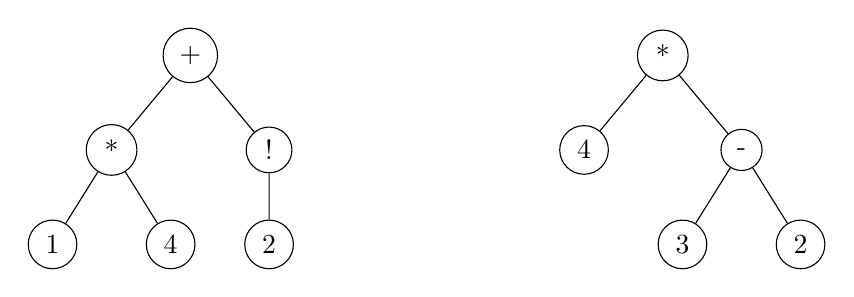
\begin{tikzpicture}[level distance=1.2cm,
    level 1/.style={sibling distance=2cm},
    level 2/.style={sibling distance=1.5cm}]

    \node[circle,draw] {+}
        child { 
            node[circle,draw] {*} 
            child { node[circle,draw] {1} }
            child { node[circle,draw] {4} }
        }
        child { 
            node[circle,draw] {!}
            child { 
                node[circle,draw] {2}
            }
        };

    \begin{scope}[xshift=6cm]

        \node[circle,draw] {*}
            child { 
                node[circle,draw] {4} 
            }
            child { 
                node[circle,draw] {-}
                child { node[circle,draw] {3} }
                child { node[circle,draw] {2} }
            };

    \end{scope}
\end{tikzpicture}
\vspace{0.4cm}